\clearpage
\section*{3. Proposed Approach}
\label{sec:approach}
\subsection*{3.1 Design principles}

The proposed solution introduces the smallest state needed to connect congestion-window growth to actual flight history. State is stored per path because bytes in transit and CUBIC state are already path specific. The feature is optional so that the original behaviour can be used for compatibility checks. Its activation string is rli=on with CUBIC selected. DCUBIC has a separate initializer that keeps RLI disabled despite sharing controller machinery \cite{ref12}.


Each path records maxFS, the currently computed limit, a cap-active flag, and a saturating reset counter. On initialization, maxFS is set to the source's initial window. After a send or removal changes bytes\_in\_transit, the accounting helper retains the larger of the existing maximum and the new flight size. On a genuine cwnd reduction, the helper clears maxFS and the cached cap state, and increments the reset counter. Subsequent flight updates rebuild the observation history.


\subsection*{3.2 Candidate growth and limiting rule}

The growth candidate remains part of the existing controller. In RLI slow start, the implementation obtains the normal target-window estimate and adds newly acknowledged bytes using saturating addition. This bypasses a legacy helper gate that would otherwise suppress the very application-limited growth under investigation. In congestion avoidance, the controller computes the cubic and Reno-friendly candidates and selects the larger. Epoch adjustment for a sender-limited interval remains in place.



\begingroup\footnotesize
\begin{verbatim}
L_SS = saturating_multiply_by_two(maxFS)
L_CA = saturating_add(maxFS, send_mtu)
bounded_candidate = min(candidate, L_phase)
cwnd_after_ACK = max(cwnd_before_ACK, bounded_candidate)
\end{verbatim}
\endgroup

The final maximum with the previous window is essential: the limiter constrains increases rather than creating a new congestion signal. If an epoch adjustment produces a smaller candidate, ordinary ACK processing preserves the previously permitted window. Real loss, ECN, timeout, or startup congestion responses remain responsible for reductions and observation resets. The implementation then clips W\_reno to avoid leaving an internal window estimate above the exposed result.





\clearpage
\subsection*{3.3 Controlled topology}

\begin{center}
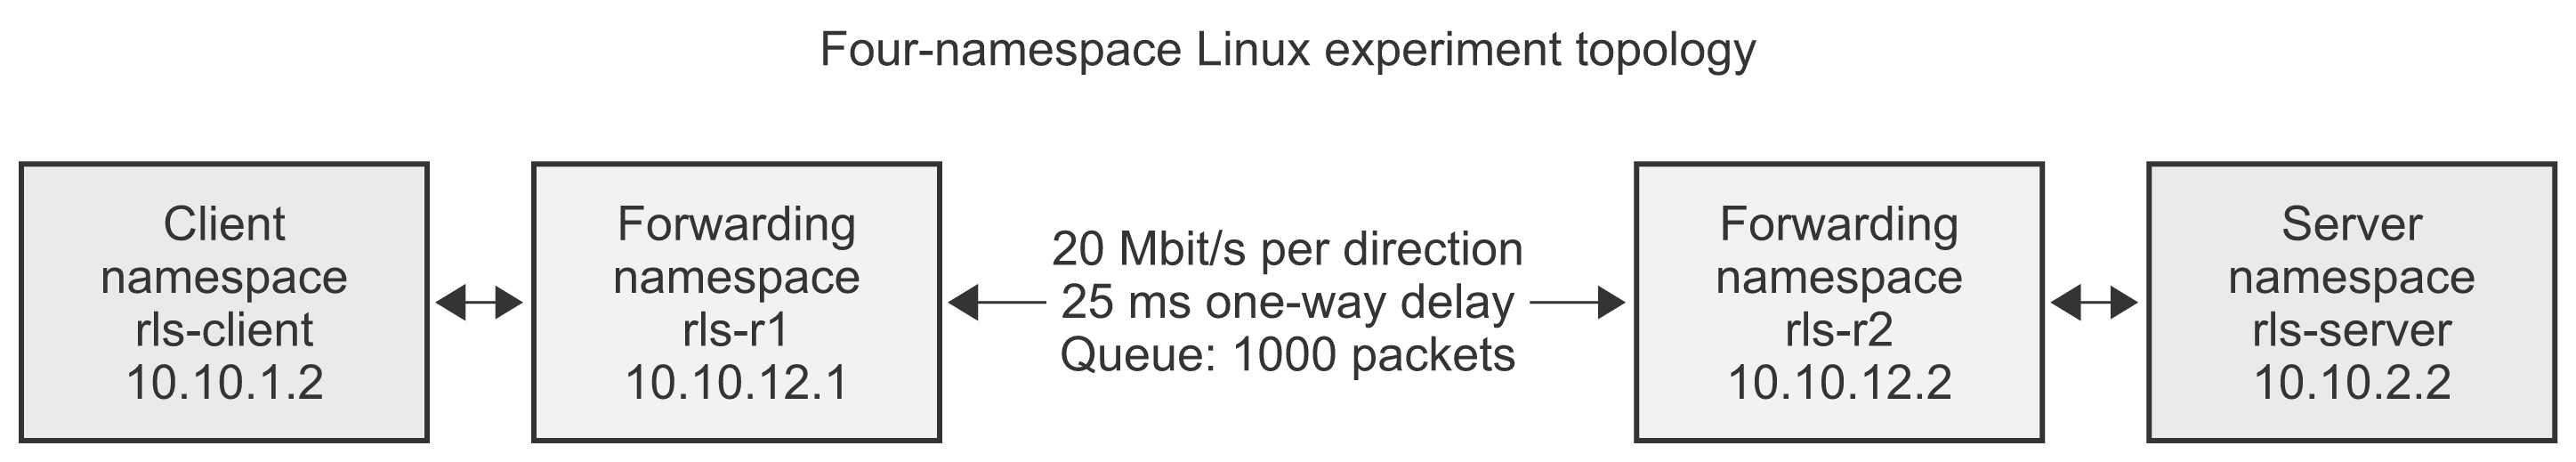
\includegraphics[width=\linewidth,height=0.48\textheight,keepaspectratio]{images/topology.png}
\captionof{figure}{Four-namespace Linux experimental topology. The server sends the measured payload to the client.}
\end{center}


The main topology has two endpoint namespaces and two forwarding namespaces. The core link carries 20 Mbit/s in each direction with 25 ms of one-way delay and a 1000-packet queue limit. The base round-trip time is approximately 50 ms. The supplementary dumbbell connects two client/server pairs across the same shaped link. Each supplementary run starts both transfers together \cite{ref12,ref13}.

\subsection*{3.4 Traceability and analysis}

Each run records the command, binary identity, configuration, performance data, and qlog traces. The source revision for the actual baseline binary is recorded in its \path{provenance.txt}. The sender qlog provides the window and flight-size samples. The server connection CSV supplies byte counts and connection times. The analysis weights each window sample by the time until the next sample. The comparison reports the means and sample variability across the three repetitions.

\label{sec:approach-end}
